\documentclass[11pt,a4paper]{article}
\usepackage{paramanu}
\usepackage{multicol}
\usepackage{titlesec}
\titlespacing*{\section}{0pt}{11pt plus 3pt minus 2pt}{5pt plus 1pt}
\titlespacing*{\subsection}{0pt}{8pt plus 2pt minus 2pt}{3pt plus 1pt}

% Theorem-like environments (kept here so the Word converter can number them).
% Link to a file in the public repository (the evidence behind a claim).
\newcommand{\repourl}{https://github.com/syncaissa/paramanu-reclaimer}
\newcommand{\gh}[2]{\href{https://github.com/syncaissa/paramanu-reclaimer/blob/main/#1}{\texttt{#2}}}

\theoremstyle{definition}
\newtheorem{definition}{Definition}[section]
\theoremstyle{plain}
\newtheorem{proposition}{Proposition}[section]
\theoremstyle{remark}
\newtheorem*{remark}{Remark}

\setrunningtitle{PARAMANU Reclaimer: Atomize-First Recovery from Landfill to the Periodic Table}
\hypersetup{pdftitle={PARAMANU Reclaimer: Atomize-First Recovery -- A Sealed Plasma Reactor from Landfill to the Periodic Table},
  pdfauthor={Milind K. Patil}}

% Let floats fill pages densely (avoids half-empty pages before large tables).
\renewcommand{\topfraction}{0.9}
\renewcommand{\bottomfraction}{0.8}
\renewcommand{\textfraction}{0.07}
\renewcommand{\floatpagefraction}{0.75}
\setcounter{topnumber}{3}
\setcounter{totalnumber}{5}
\setlength{\textfloatsep}{10pt plus 2pt minus 3pt}
\setlength{\floatsep}{8pt plus 2pt minus 2pt}
\setlength{\intextsep}{8pt plus 2pt minus 2pt}
\AtBeginDocument{\setlength{\abovedisplayskip}{6pt plus 2pt minus 2pt}\setlength{\belowdisplayskip}{6pt plus 2pt minus 2pt}}

\begin{document}
\thispagestyle{plain}

\begin{ptitle}
PARAMANU RECLAIMER: PLASMA-ASSISTED RECOVERY AND MINING OF ATOMS, NEUTRALIZING URBAN-WASTE
\end{ptitle}

\begin{psubtitle}
Atomize-First Recovery: A Sealed Plasma Reactor\\
from Landfill to the Periodic Table
\end{psubtitle}

\begin{pauthor}
Milind K. Patil\\
Syncaissa Systems Inc.\\
\texttt{syncaissa@outlook.com}
\end{pauthor}

\begin{pdate}
September 2026
\end{pdate}

\begin{pabstract}
Every recycling system today follows one rule: \emph{sort first}. The fine, mixed residue that sorting cannot handle, most of an old landfill, is capped, burned or buried again. The \textbf{PARAMANU Reclaimer} (Plasma-Assisted Recovery And Mining of Atoms, Neutralizing Urban-waste) starts where sorting ends: a sealed, stack-free plasma reactor turns the residue fully into gas, and condensers at falling temperatures separate its elements band by band. We call this architecture \textbf{Atomize-First}. We derive eight design principles from established thermodynamics, with proofs, and test the design with an open simulation on NASA data, a 5,000-feed sweep and repeated rechecks of the computation. The results support it, placing valuable and toxic volatile metals in different bands, and correct it: the hot zone must last only tens of milliseconds, and mercury needs its own trap. \emph{Fume}, fine particles that can carry metals past their condenser, is the largest open threat. Predictions registered before any experiment will judge a working plant. All code and data are public.
\begin{pkeywords}
\textbf{Keywords:} atomize-first recovery, sealed plasma reactor, plasma heap, condensation ladder, atomic recycling, landfill mining, residual waste, zero-stack process, closed-mass principle, internal reductant, periodic-table recovery, value--harm slider, Gibbs-energy minimization, verification certificate, pre-registration
\end{pkeywords}
\end{pabstract}

\begin{execsummary}
\textbf{The idea:} PARAMANU starts where sorting stops, vaporizing unsortable residue in a sealed reactor and collecting each element as the gas cools (\emph{metals mined once, harvested again}); every atom exits through a labelled outlet; no process gas is vented. \textbf{What is proven:} eight design principles from established thermodynamics, with proofs. \textbf{What the simulation shows:} all gas at about 2,890\,K for 2.9\,MWh per tonne; Pd and Pt follow iron, and gold splits between the iron and copper bands; in 5,000 feeds no zinc, mercury or lead, and at most 0.01\% of the cadmium, reaches a gold band; half the mercury needs a trap; the hot zone lasts only tens of milliseconds. \textbf{How it was rechecked:} all 570,000 states pass a certificate, a second solver and database agree, an adversary broke the first lead design, fixed by a band split, and results reproduce to $10^{-13}$. \textbf{Energy:} a dedicated power plant is needed; fuel, steam and sales (\$113 per tonne) cover 40--50\% of the power bill; self-sufficiency needs twice today's heating efficiency. \textbf{What remains:} whether a real reactor, especially its fume, matches the model; thirteen pre-registered predictions will decide.
\end{execsummary}

\section{Introduction}

Landfills hold decades of metals, critical elements and toxic substances mixed with soil, plastics and organic matter. Research treats them as ``anthropogenic resources'' \citep{krook2012,winterstetter2015}, and enhanced landfill mining (ELFM) adds energy recovery to material recovery \citep{jones2013}. Projects work when the target is simple: a metals-only project at a Maine ashfill recovered 34,352\,t of metals worth about US\$7.4 million \citep{wagner2015}. Nearly all approaches follow one rule, \textbf{sort first}: crush, then separate by magnets, eddy currents, screens and optical sensors. Sorting fails for the residue: the fines, composites, ash and smeared mixtures that no machine can tell apart. That residue is the largest stream in excavated landfill material \citep{quaghebeur2013,hernandez2018} and holds most trace metals and toxic elements, which is why 34 of 60 metals are still recycled below 1\% \citep[Fig.~4]{graedel2011}.

This paper asks: \emph{if recovery must eventually work at the atomic level, why sort objects at all?} Once residue is turned into atoms in a closed vessel, a pizza box and a battery are the same thing: a mixture of elements that physics can separate by the temperatures at which they condense. We call this approach \textbf{Atomize-First}, and its system the \textbf{PARAMANU Reclaimer}. \emph{Param\={a}\d{n}u} is Sanskrit for the atom, the ``ultimate particle'' of classical Indian philosophy. The metals in a landfill were \emph{mined once}, from ore, at great cost to the land; PARAMANU \emph{harvests them again}, from the waste we buried.

\begin{figure}[!htbp]
\centering
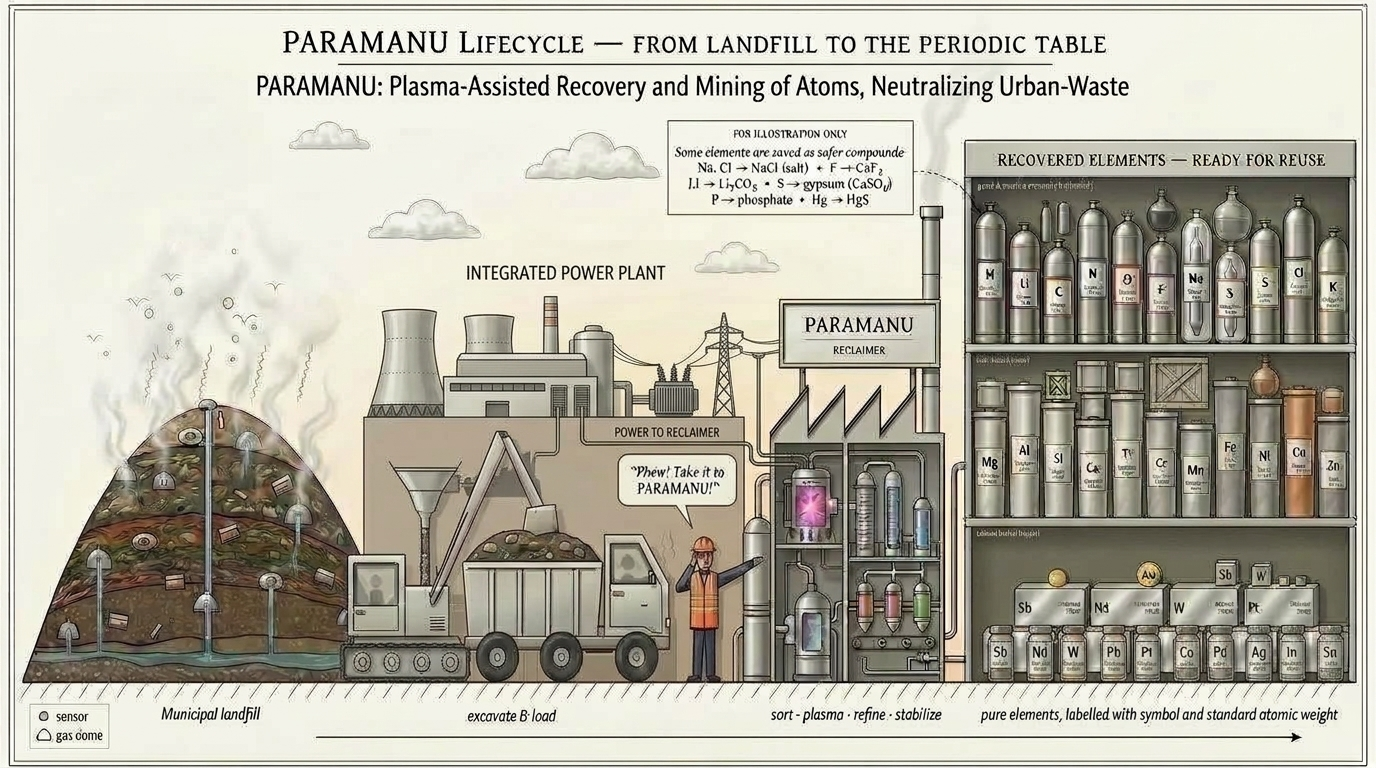
\includegraphics[width=0.78\textwidth]{figures/paramanu_lifecycle_good_with_powerplant.png}
\caption{The PARAMANU lifecycle, from landfill to the periodic table (illustrative). A dedicated power plant supplies the Reclaimer; recovered elements are stored pure or, where the pure element is reactive or toxic, as stable compounds, on shelves labelled with their symbols and standard atomic weights.}\label{fig:lifecycle}
\end{figure}

\textbf{Scope.} How much existing pre-treatment (magnets, eddy currents) comes first is left to the implementer. It is encouraged, because it mainly lowers the energy bill; product purity is set by the atomic separation. Only making hazards safe is mandatory: batteries, cylinders and aerosol cans are discharged and dismantled, and radioactive items go to a licensed handler (Section~\ref{sec:safety}).

\paragraph{Contributions.}
\begin{enumerate}[nosep,leftmargin=*]
\item The \textbf{Atomize-First architecture}, a sealed plasma reactor with no stack in which the residue becomes a ``plasma heap'', and the \textbf{closed-mass principle} (Section~\ref{sec:arch}).
\item The \textbf{condensation ladder} and the \textbf{internal reductant}: the waste's own carbon and hydrogen bind its oxygen, so metals condense as metals (Section~\ref{sec:arch}).
\item \textbf{Eight design principles} from established thermodynamics, with proofs, applied for the first time to atomic recovery from waste, and an \textbf{implementer's guide} (Section~\ref{sec:math}, Appendix~A).
\item A \textbf{reference plant} tying each station to its governing result and its test (Section~\ref{sec:walk}).
\item \textbf{Open computational evidence} and a 5,000-feed sweep that confirm, correct and extend the vision (Section~\ref{sec:evidence}).
\item \textbf{Rechecks of the computation} and \textbf{pre-registered predictions} (Section~\ref{sec:verification}).
\item An \textbf{energy account}, including self-sufficiency (Section~\ref{sec:energy}).
\item A \textbf{value--harm policy}, a \textbf{Sort-First baseline}, what is proven and open, and a \textbf{research agenda} (Sections~\ref{sec:safety}--\ref{sec:feasibility}).
\end{enumerate}

\textbf{Open evidence.} Every number, figure and check here comes from public code and data at \url{https://github.com/syncaissa/paramanu-reclaimer}. Each script or file named in the text links to it, and \gh{Results.txt}{Results.txt} lists every result with the script that produced it.

\section{Background}\label{sec:background}

\textbf{Landfill mining} has two decades of history \citep{krook2012}; fines are its largest and hardest stream \citep{quaghebeur2013,hernandez2018,burlakovs2018}, precious metals in landfill cores are below ore grade \citep{gutierrez2015}, and its economics rest on gate fees, energy and material revenue \citep{laner2019}. \textbf{Thermal plasma} gasifies organics and melts inorganics into glass \citep{heberlein2008,gomez2009,bosmans2013}, but it does not separate elements, and it carries real risk, as the US\$0.9--1.0 billion Tees Valley write-down showed \citep{icheme2016}. \textbf{Metals in waste} are spread thin through ash \citep{morf2013}, electronics \citep{cui2008} and even wastewater (Swiss wastewater carries about 43\,kg of gold and 3,000\,kg of silver a year; \citealp{vriens2017}), and recovery cost rises steeply as concentration falls \citep{sherwood1959,johnson2007}. \textbf{Separation after decomposition} exists in parts: flash Joule heating evaporates precious metals from e-waste in milliseconds \citep{deng2021}, plasma mass filters separate by mass \citep{gueroult2015,zweben2018}, and zinc smelting condenses metal vapors \citep{cusano2017bref}; none treats a whole mixed residue. The idea itself is old: Eastlund and Gough's \emph{fusion torch} proposed breaking any waste into its elements in the plasma of a fusion reactor \citep{eastlund1969}, but it stayed a concept. To our knowledge, PARAMANU is the first quantitative, computationally checked design of that idea, with conventional plasma torches and separation by condensation (Table~\ref{tab:prior}).

\begin{table}[!htbp]
\centering
\caption{PARAMANU among related approaches. ✓ present, ✗ absent, ∼ partial. The PARAMANU row states design intent.}\label{tab:prior}
\footnotesize\setlength{\tabcolsep}{4.5pt}
\begin{tabular}{@{}lcccccc@{}}
\toprule
\textbf{Approach} & \textbf{Mixed} & \textbf{Unsorted} & \textbf{Atomic} & \textbf{No} & \textbf{Element} & \textbf{Toxic} \\
 & \textbf{residue} & \textbf{feed} & \textbf{separation} & \textbf{stack} & \textbf{bands} & \textbf{capture} \\
\midrule
Landfill mining / ELFM & ∼ & ✗ & ✗ & ✗ & ✗ & ∼ \\
Plasma ELFM & ✓ & ∼ & ✗ & ✗ & ✗ & ✓ \\
Incinerator ash recovery & ✓ & ✗ & ✗ & ✗ & ✗ & ∼ \\
Fusion torch (1969 concept) & ✓ & ✓ & ✓ & ∼ & ∼ & ∼ \\
Flash Joule heating & ✗ & ✗ & ✓ & ∼ & ∼ & ✓ \\
Plasma mass filter & ✗ & ✗ & ✓ & ✓ & ∼ & ✗ \\
\textbf{PARAMANU} & ✓ & ✓ & ✓ & ✓ & ✓ & ✓ \\
\bottomrule
\end{tabular}
\end{table}

\section{The Atomize-First Architecture}\label{sec:arch}

The architecture has three stages (Figure~\ref{fig:atomize}). \textbf{Stage~0, pre-treatment,} is the implementer's choice, except that hazards are always made safe; the residue is then dried with waste heat. \textbf{Stage~1, the sealed hot zone:} the residue enters through an argon-purged lock, and plasma torches turn all of it into gas, the ``plasma heap'' (a torch-heated vapor, only 0.02\% ionized). The trash has no structure left, and with no chimney its ``smoke'' stays in the heap. \textbf{Stage~2, atomic separation:} as the gas cools, tungsten and titanium condense first; then iron, with palladium, platinum, cobalt and part of the gold; then silicon, nickel and copper, with the rest of the gold; then salts, silver and lead; and zinc and cadmium near the cold end, far from the gold. Mercury goes to a trap, the fuel gas to a fuel line, and what is not worth purifying is vitrified as future ore.

\begin{figure}[!htbp]
\centering
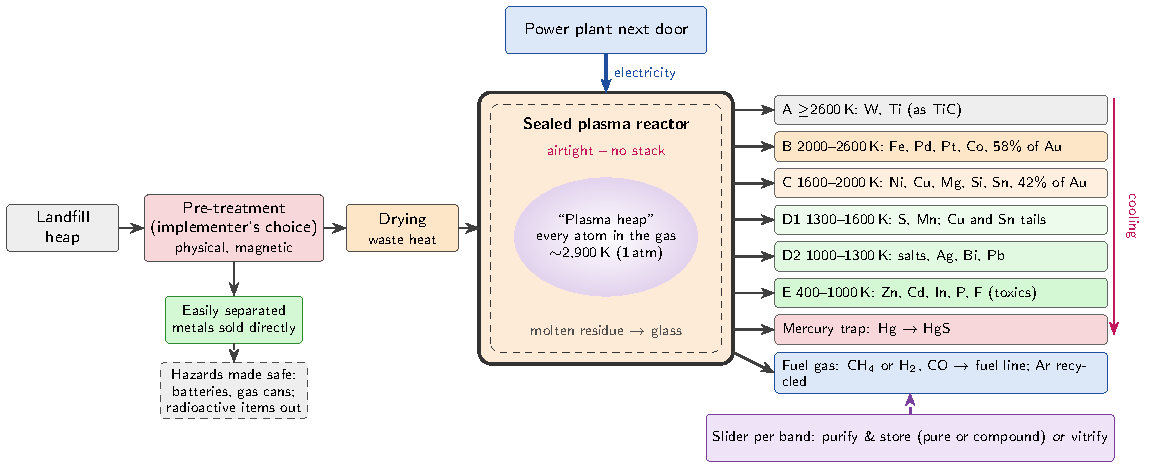
\includegraphics[width=\textwidth]{figures/fig_atomize.pdf}
\caption{The Atomize-First architecture. Pre-treatment (its extent left to the implementer) removes easily separated metals and always makes hazards safe; the dried residue is sealed in an airtight plasma reactor with no stack; as the gas cools, elements are harvested in the simulated condensation bands, mercury in a trap, and the fuel gas drawn off to a fuel line. The value--harm slider decides, band by band, what is purified and what is vitrified.}\label{fig:atomize}
\end{figure}

\begin{algorithm}[!htbp]
\caption{Atomize-First cycle for one parcel of residue, from sealed hot zone to separated elements}\label{alg:batch}
\begin{algorithmic}[1]
\Require Pre-treated, dried residue; condenser temperatures $T_{\mathrm{A}} > T_{\mathrm{B}} > T_{\mathrm{C}} > T_{\mathrm{D1}} > T_{\mathrm{D2}} > T_{\mathrm{E}}$ set for the operating pressure from the simulated bands (Result~3); slider $s$
\Ensure Band condensates $\{B_k\}$, trap product, fuel gas, glass; no process gas vented
\State Feed the residue through the argon-purged lock into the sealed train
\State Raise each parcel to the all-gas state in the hot zone, for at most tens of milliseconds \Comment{Result~5}
\For{each band $k = \mathrm{A, B, C, D1, D2, E}$}
  \State Pass the parcel through condenser $k$ held at $T_k$; harvest condensate $B_k$
  \State Filter the fume leaving stage $k$ and return it to $B_k$
  \For{each element $i$ in $B_k$}
    \If{$V_i + s H_i > C_i$} \State send $i$ to purification; store pure or as a stable compound
    \Else \State send $i$ to vitrification \Comment{future ore}
    \EndIf
  \EndFor
\EndFor
\State Capture mercury in the sulfur-impregnated carbon trap; separate the water condensate
\State Compress the remaining gases (CH$_4$, or H$_2$ and CO if quenched; N$_2$) to the fuel line; recycle Ar
\State Tap the molten mineral residue to vitrification; close every element balance over the outlets \Comment{Result~1}
\end{algorithmic}

\end{algorithm}

\begin{definition}[Closed-mass principle]
A PARAMANU reactor satisfies the closed-mass principle if every atom that enters leaves through one of a finite set of labelled outlets: a condensation band collector, a fume filter, a trap, the water condensate, the fuel-gas line or the vitrified residue. No outlet discharges to the atmosphere, and each outlet is a product or a stream that must itself be treated.
\end{definition}

The principle turns ``do we capture the smoke?'' into a design rule: there is no smoke, only product streams not yet harvested. It governs the process; burning the fuel and making the electricity have their own stacks, counted in the life-cycle account (Section~\ref{sec:safety}). The vision pictured one sealed batch cooling slowly; Result~5 rules that out. The reference design keeps the physics and changes the geometry: residue flows through a sealed train (a millisecond hot zone, then condensers at falling temperatures), so every parcel of gas is its own batch, heated once and cooled once, and the ladder is laid out in space rather than in time.

\textbf{The ladder, as first envisioned.} By boiling point the elements fall into five bands: tungsten, platinum and titanium above 3,500\,K; iron, gold, palladium, nickel and copper at 2,800--3,500\,K; aluminium, silver and lead at 2,000--2,800\,K; zinc, cadmium, magnesium and the alkali metals at 1,000--2,000\,K; and mercury, sulfur and phosphorus below 1,000\,K \citep{crc2014}. The vision rested on two hopes, that \emph{the volatile toxic metals separate from the valuable ones} and that \emph{the ladder concentrates traces} (Figure~\ref{fig:ladder}); Section~\ref{sec:evidence} tests both.

\begin{figure}[!htbp]
\centering
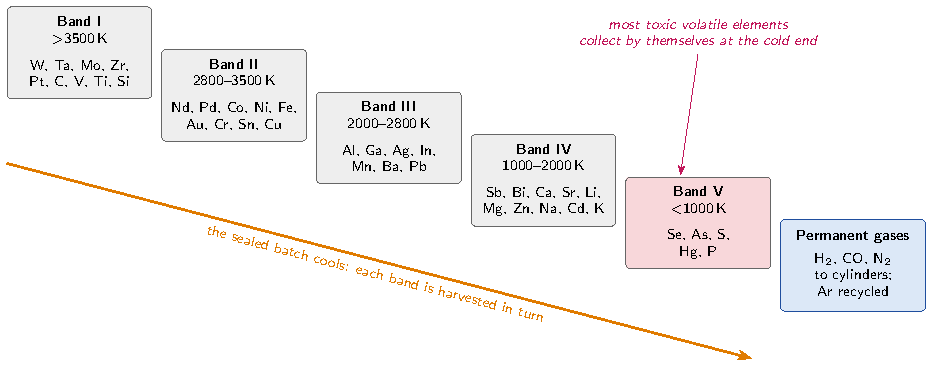
\includegraphics[width=0.72\textwidth]{figures/fig_ladder.pdf}
\caption{The condensation ladder as first conceived, in time; the reference design lays it out in space (Section~\ref{sec:walk}).}\label{fig:ladder}
\end{figure}
 Both survive, at temperatures far below the boiling points. Neighbours such as iron, nickel, copper and gold still condense together as an alloy, so established refining finishes the job; a plasma mass filter, separating by mass rather than volatility \citep{gueroult2015,zweben2018}, could one day split such groups.

\textbf{The heap carries its own reducing agent.} If oxygen recombines with metals during cooling, the bands hold oxides; the waste's plastics and paper supply the remedy.

\begin{proposition}[Internal reductant capacity]\label{prop:reductant}
If each carbon atom can bind one oxygen atom as CO and each pair of hydrogen atoms one oxygen atom as H\textsubscript{2}O, then with silica, polyethylene and cellulose as proxies for soil and glass, plastics and paper, the residue of one wet tonne has an oxygen-binding capacity of
\begin{equation}\label{eq:reductant}
\frac{n_{\mathrm{C}} + n_{\mathrm{H}}/2}{n_{\mathrm{O}}} = \frac{12{,}955 + 24{,}799/2}{18{,}254} \approx 1.39 .
\end{equation}
\end{proposition}
\begin{proof}
The mole numbers follow from the proxy compositions and masses; the ratio is direct arithmetic.
\end{proof}

With the full feed model the ratio is 1.52, and in the simulation iron condenses entirely as metal, against 43\% without the organics (Section~\ref{sec:evidence}).

\section{Design Principles from Established Thermodynamics}\label{sec:math}

Mathematics cannot prove that a plant works; only experiments can. It can show what physics permits and turn those limits into design equations. \textbf{None of the mathematics below is new}: conservation of mass (Result~1), Gibbs-energy minimization \citep{gordon1994,boyd2004} (Results~2 and~7), Clausius--Clapeyron (Result~3), the Fenske equation (Result~4), grey-body radiation with the isoperimetric inequality (Result~5), the ideal entropy of mixing (Result~6) and detailed balance (Result~8). What is new is their use in atomic recovery from waste, where each becomes a design rule, a sizing number or an acceptance test. We give each proof, and each result is checked against the full simulation on GitHub (\gh{simulation/scripts/07_theory_checks.py}{07\_theory\_checks.py}, \gh{simulation/tests/test_theory.py}{test\_theory.py}). Throughout, $T$ is temperature, $P$ pressure, $P_0 = 1$\,atm, $R$ the gas constant, $n_i$ the moles of element $i$, $a_k$ the atoms in species $k$, and $g_k = G^\circ_k/RT$.

\subsection{Result 1: Every Atom Is Accounted For}
\begin{proposition}[Closed-mass balance]\label{prop:closedmass}
If the closed-mass principle holds, then for every element over a batch or a period of steady operation, with $\mathcal{O}$ the set of outlets,
\begin{equation}\label{eq:closedmass}
\textstyle\sum_{o\in\mathcal{O}} n_{i,o} = n_i^{\mathrm{in}}.
\end{equation}
\end{proposition}
\begin{proof}
Reactions rearrange atoms but neither create nor destroy them. The principle removes every path to the atmosphere, and at steady state (or at the end of a batch) the reactor inventory is unchanged.
\end{proof}
This is conservation of mass; we state it because Eq.~\ref{eq:closedmass} becomes the first acceptance test of a real plant.

\subsection{Result 2: The Equilibrium Exists and Is Unique}
\begin{proposition}[Existence and uniqueness]\label{prop:unique}
For an ideal gas, any number of pure condensed phases and any number of ideal solutions at fixed $T$ and $P$, the minimum of the Gibbs energy subject to the element balances exists. The composition of the gas and of each solution at the minimum is unique, and the element potentials $\lambda$ solve the concave dual problem
\begin{equation}\label{eq:dual}
\max_{\lambda}\; \textstyle\sum_i n_i\lambda_i \quad \text{s.t.}\quad \sum_{k\in\mathrm{gas}} e^{\,a_k\cdot\lambda - g_k - \ln(P/P_0)} \le 1,\quad \sum_{k\in s} e^{\,a_k\cdot\lambda - g_k}\le 1,\quad a_c\cdot\lambda \le g_c,
\end{equation}
where $s$ runs over the solutions and $c$ over the pure phases.
\end{proposition}
\begin{proof}
The feasible set $\{\mathbf{n}\ge 0 : A\mathbf{n} = \mathbf{b}\}$ is a non-empty compact polytope and $G(\mathbf{n})$ is continuous on it, so a minimum exists. $G$ is a sum of linear terms (pure phases) and terms $N\sum_k x_k(g_k+\ln x_k)$ for each mixture, which are strictly convex in the mole fractions; hence each mixture's composition at the minimum is unique. The constraints are linear and Slater's condition holds, so strong duality gives the element potentials as multipliers. At the optimum, $\ln x_k = a_k\cdot\lambda - g_k$ (less $\ln(P/P_0)$ in the gas); summing $x_k$ to one gives the mixture constraints, and a pure phase is stable only where $a_c\cdot\lambda = g_c$ \citep{gordon1994}.
\end{proof}
The solver's answer is thus not one of several; Section~\ref{sec:certificate} turns this dual into a certificate.

\subsection{Result 3: When a Dilute Element Condenses}
\begin{proposition}[Onset of condensation]\label{prop:onset}
An element with monatomic vapor at mole fraction $y$, whose pure condensed phase has saturation pressure $p^{\mathrm{sat}}(T)$, begins to condense at $T_c$ where
\begin{equation}\label{eq:onset}
y\,P = p^{\mathrm{sat}}(T_c), \qquad \frac{1}{T_c} \approx \frac{1}{T_b} - \frac{R}{\Delta H_{\mathrm{vap}}}\ln\frac{yP}{P_0},
\end{equation}
with $T_b$ the normal boiling point. If it dissolves in a condensing host with activity coefficient $\gamma$ at mole fraction $x$, the condition is $yP = \gamma x\,p^{\mathrm{sat}}$.
\end{proposition}
\begin{proof}
Condensation begins when $\mu^\circ_{\mathrm{gas}} + RT\ln(yP/P_0)$ first equals $\mu^\circ_{\mathrm{cond}}$, and $RT\ln(p^{\mathrm{sat}}/P_0) = \mu^\circ_{\mathrm{cond}} - \mu^\circ_{\mathrm{gas}}$. Integrating Clausius--Clapeyron from $T_b$ with constant $\Delta H_{\mathrm{vap}}$ gives the closed form; a dissolved element adds $RT\ln(\gamma x)$.
\end{proof}
A dilute element condenses hundreds of kelvin below its boiling point, and every band moves with pressure (Table~\ref{tab:onset}).

\begin{table}[!htbp]
\centering
\caption{Result 3 against the simulation (default feed, 1\,atm; \gh{simulation/scripts/07_theory_checks.py}{07\_theory\_checks.py}).}\label{tab:onset}
\footnotesize
\begin{tabular}{@{}lrrrrr@{}}
\toprule
\textbf{Metal} & \textbf{$T_b$ (K)} & \textbf{$\Delta H_{\mathrm{vap}}$ (kJ/mol)} & \textbf{Closed form (K)} & \textbf{Exact (K)} & \textbf{Simulated (K)} \\
\midrule
Fe & 3139 & 349 & 2315 & 2330 & 2320 \\
Cu & 2844 & 301 & 1760 & 1774 & 1770 \\
Pb & 2022 & 178 & 1061 & 1070 & 1070 \\
Zn & 1179 & 115 & 715 & 722 & 720 \\
\bottomrule
\end{tabular}
\end{table}

\subsection{Result 4: Which Elements Physics Can Separate}
\begin{proposition}[Separation limits]\label{prop:fenske}
For two elements condensing together as one solution with constant relative volatility $\alpha = \gamma_i p_i^{\mathrm{sat}}/\gamma_j p_j^{\mathrm{sat}} > 1$: (a) one fractional condensation leaves in the gas a fraction $(1-f)^{1/\alpha}$ of $i$ when a fraction $f$ of $j$ has condensed; (b) splitting the pair into products of purity $p$ needs at least
\begin{equation}\label{eq:fenske}
N_{\min} = \ln\!\big[p^2/(1-p)^2\big]\big/\ln\alpha
\end{equation}
ideal condensation--re-evaporation stages.
\end{proposition}
\begin{proof}
(a) By Raoult's law the condensate has $x_i/x_j = (1/\alpha)\,n_i/n_j$, so $dn_i/dn_j = (1/\alpha)\,n_i/n_j$, which integrates to $n_i/n_i^0 = (n_j/n_j^0)^{1/\alpha}$. (b) Each ideal stage multiplies $y_i/y_j$ by $\alpha$; going from $(1-p)/p$ to $p/(1-p)$ needs $\alpha^N = p^2/(1-p)^2$ (the Fenske equation).
\end{proof}
With NASA vapor pressures, zinc, magnesium and mercury leave iron in one stage, lead leaves copper in 1.5, silver leaves gold in 2 and cadmium leaves zinc in 5, but gold from iron ($\alpha = 1.43$) needs 26 (\gh{simulation/scripts/07_theory_checks.py}{07\_theory\_checks.py}). \textbf{Physics separates the toxic volatile metals from the precious ones, not gold or palladium from iron}; that step belongs to established refining \citep{cui2008}.

\subsection{Result 5: How Briefly the Heap Must Be Hot}
\begin{proposition}[Hot-zone design laws]\label{prop:hotzone}
Let the feed need specific energy $e$ to reach the all-gas state at $T$ and $P$, forming $\nu$ moles of gas per kilogram, radiating as a grey body of emissivity $\varepsilon$ to walls at $T_w$. (1) A batch of mass $m$ radiates its own energy in
\begin{equation}\label{eq:tau}
\tau = \frac{e\,m}{\varepsilon\sigma\,(36\pi)^{1/3}\,(\nu m R T/P)^{2/3}\,(T^4 - T_w^4)} \;\propto\; m^{1/3}P^{2/3}.
\end{equation}
(2) A continuous hot zone processing $\dot m$ with residence time $t_r$ loses the fraction
\begin{equation}\label{eq:flowloss}
\frac{Q}{\dot W} = \frac{\varepsilon\sigma(36\pi)^{1/3}\,(\dot m\,\nu R T t_r/P)^{2/3}\,(T^4-T_w^4)}{\dot m\,e} \;\propto\; t_r^{2/3}\,\dot m^{-1/3}
\end{equation}
of its power to radiation. For a given $\varepsilon$ both are best cases.
\end{proposition}
\begin{proof}
The gas fills $V = \nu m RT/P$. The smallest surface enclosing $V$ is a sphere of area $(36\pi)^{1/3}V^{2/3}$ (isoperimetric inequality), and grey-body exchange gives $Q = \varepsilon\sigma A(T^4-T_w^4)$, so $\tau = em/Q$. In continuous flow $V = \dot m\,\nu RT t_r/P$ and $\dot W = \dot m e$.
\end{proof}
Result~5 is an order-of-magnitude estimate: $\varepsilon$ and convection must be measured, and particle-laden gas ($\varepsilon \to 1$) loses about three times more (Section~\ref{sec:practical}). With simulated values ($e = 9.8$\,MJ/kg, $\nu = 35.1$\,mol/kg, $T = 2{,}890$\,K), a one-tonne batch radiates its own energy in $\tau \approx 4.2$\,s (\gh{simulation/scripts/08_reactor_design.py}{08\_reactor\_design.py}): as gas it would fill a sphere 28\,m across and radiate 1--3\,GW against a batch energy of 4\,MWh. A slowly cooled batch is impractical at every size from 1\,kg to 10\,t. A flow is not: at 1,000 tonnes per day radiation stays below 10\% of torch power for residence times up to 25\,ms, and larger plants do better ($\dot m^{-1/3}$). \textbf{This is the most important constraint the analysis added}, and it is not exotic: flash Joule heating reaches about 3,400\,K in under 50\,ms \citep{deng2021} (Figure~\ref{fig:reactordesign}).

\begin{figure}[!htbp]
\centering
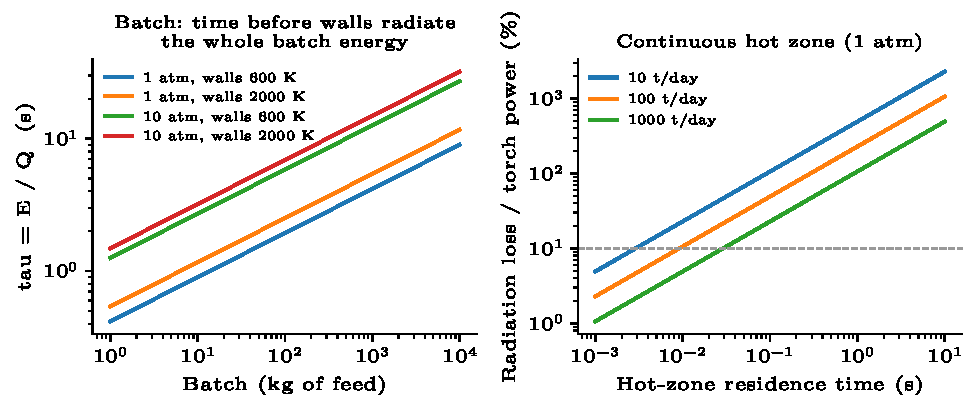
\includegraphics[width=0.84\textwidth]{figures/fig_reactor_design.pdf}
\caption{Result 5. Left: radiation time constant of a sealed batch. Right: radiation loss of a continuous hot zone against residence time.}\label{fig:reactordesign}
\end{figure}

\subsection{Result 6: Unmixing Itself Is Cheap}
\begin{proposition}[Floor on the work of separation]\label{prop:minwork}
Unmixing an ideal mixture of atoms into pure elements at $T_0$ needs at least $W_{\min} = -RT_0 \sum_i n_i \ln x_i$, with $x_i = n_i/\sum_j n_j$.
\end{proposition}
\begin{proof}
The Gibbs energy of ideal mixing is $RT_0\sum_i n_i\ln x_i<0$; by the second law, reversing it needs at least that much work.
\end{proof}
For the default feed $W_{\min} = 0.067$\,MWh per tonne, 2.3\% of the vaporization energy (\gh{simulation/scripts/07_theory_checks.py}{07\_theory\_checks.py}). The energy goes into heating and the walls, not unmixing, so efficiency work belongs to heat delivery and recovery.

\subsection{Result 7: The Heap Forgets What It Was}
\begin{proposition}[Structure independence]\label{prop:structure}
At fixed $T$ and $P$, the equilibrium of a closed batch depends on its feed only through the element totals. Feeds with equal totals, whatever molecules they contain, reach the same state.
\end{proposition}
\begin{proof}
$G(\mathbf{n})$ is minimized subject to $A\mathbf{n} = \mathbf{b}$; neither refers to the feed's molecules, which enter only through $\mathbf{b}$. By Result~2 the minimum is unique.
\end{proof}
Atomize-First is therefore indifferent to the complexity of waste, from pharmaceuticals to PFAS: sorting by molecule becomes accounting by element. Three very different mixtures with equal totals reach the same state to $10^{-11}$ in a second, separately written solver, and at 2,890\,K CF\textsubscript{4} is at $10^{-38}$ and naphthalene at $10^{-28}$ (\gh{simulation/scripts/13_breakdown.py}{13\_breakdown.py}).

\subsection{Result 8: A Catalyst Cannot Change the Outcome}
\begin{proposition}[Catalyst invariance]\label{prop:catalyst}
A catalyst that is not consumed changes no equilibrium constant, and so leaves the equilibrium of the heap unchanged at every $T$ and $P$. A catalyst that is consumed acts only through the element totals it adds.
\end{proposition}
\begin{proof}
$K = e^{-\Delta_r G^\circ/RT}$ depends only on state functions of reactants and products; a catalyst appears on both sides \citep{laidler1996}. Equivalently, lowering the transition-state energy multiplies forward and reverse rate constants by the same factor, so $k_f/k_r = K$ is unchanged (detailed balance). The unique minimum of Result~2 is therefore unchanged, and a consumed catalyst enters only through $\mathbf{b}$ (Result~7).
\end{proof}
A catalyst could only speed the approach, and in the hot zone none is needed or would survive: CF\textsubscript{4} lives 80\,\textmu s at 2,890\,K \citep{modica1968,cobos2023}, over 300 lifetimes in 25\,ms, and a 5\,nm nickel particle evaporates in 2.4\,\textmu s (\gh{simulation/scripts/17_catalysts.py}{17\_catalysts.py}). The slow step, heating mineral grains, is sped up by finer grinding, hydrogen-rich gas and the waste's own carbon, which lowers the vaporization temperature of silica by about 1,100\,K. Catalysts belong at the cold end, below about 1,000\,K, for tar reforming, dioxin destruction and gas upgrading after dust, halides and sulfur are removed \citep{argyle2015,neuwahl2019}. Two rules protect the environment there: quench from 450 to below 200\,\textdegree C within about a second, because dioxins re-form on dust near 350\,\textdegree C \citep{epa2006dioxin}; and send mercury to its sulfur trap, since catalytic oxidation of mercury needs an oxidizing gas \citep{ji2022}.

\section{The Reference Plant: From Hardware to Proof}\label{sec:walk}

Figure~\ref{fig:chamber} follows one parcel through a reference plant treating 1,000 tonnes of excavated material per day at 1\,atm, and Table~\ref{tab:walk} gives each station's governing result, design number and verifying measurement. Passing the stage held at $T$ is exactly one step of the simulated ladder, so train and ladder are the same calculation if three measurable conditions hold: \textbf{plug flow} (tracer residence time), \textbf{equilibrium in each stage} (exit gas against Result~3) and \textbf{condensate stays out} (collector balances against Result~1).

\begin{figure}[!htbp]
\centering
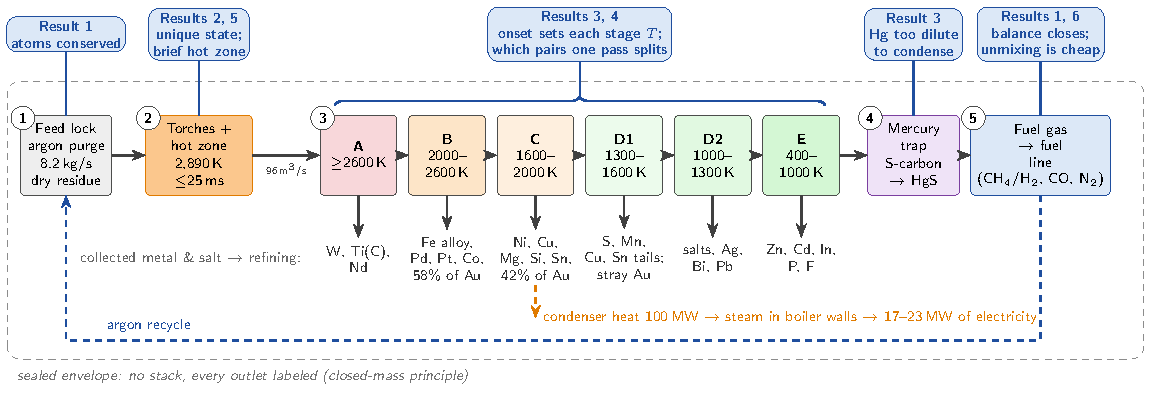
\includegraphics[width=\textwidth]{figures/fig_chamber.pdf}
\caption{The reference plant (1,000 tonnes per day, 1\,atm) and the result that governs each station. The whole train is one sealed envelope. Band temperatures are simulated at 1\,atm and move with pressure.}\label{fig:chamber}
\end{figure}

\begin{table}[!htbp]
\centering
\caption{The plant, station by station (design numbers from \gh{simulation/scripts/08_reactor_design.py}{08\_reactor\_design.py} and \gh{simulation/scripts/24_heat_recovery_and_scale.py}{24\_heat\_recovery\_and\_scale.py}).}\label{tab:walk}
\footnotesize
\begin{tabular}{@{}p{2.1cm}p{1.1cm}p{5.6cm}p{4.9cm}@{}}
\toprule
\textbf{Station} & \textbf{Result} & \textbf{Design number} & \textbf{Verified by measuring} \\
\midrule
1 Feed lock & 1 & 8.2\,kg/s dry residue; no outlet to air & every element balance closes \\
2 Hot zone & 2, 5 & 2,890\,K; 113\,MW gross ($\sim$280\,MW at demonstrated efficiency); 96\,m\textsuperscript{3}/s; $\le$25\,ms, 2.4\,m\textsuperscript{3} & exit gas vs equilibrium; wall flux vs Eq.~\ref{eq:flowloss} \\
3 Condensers & 3, 4 & six stages A--E set by Eq.~\ref{eq:onset}, built as boiler walls; 94\,MW of heat $\to$ steam, 17--23\,MW of electricity; 5.6\,kg/s collected & onset of each metal vs Table~\ref{tab:onset}; band purity vs Result~4 \\
4 Mercury trap & 3 & 58\% of the mercury arrives as vapor at 1\,atm & Hg in trap vs in bands \\
5 Fuel gas & 1, 6 & 13.6\,mol/s of CH\textsubscript{4} (or H\textsubscript{2} and CO if quenched), N\textsubscript{2}, to a fuel line (cylinders only at pilot scale); argon recycled & C, H, N balances \\
\bottomrule
\end{tabular}
\end{table}

\subsection{Why the Plasma Chamber Will Not Melt}\label{sec:walls}
At 2,890\,K the heap is hotter than steel (about 1,800\,K), copper (1,358\,K) or almost any refractory can withstand. Yet, as in smelters, glass melters and rocket engines, no wall ever has to be as hot as the gas.
\begin{enumerate}[nosep,leftmargin=*]
\item \textbf{The walls see heat, not plasma.} The arcs attach only to electrodes or the molten bath. The grey-gas wall flux is $q = \varepsilon\sigma(T^4 - T_w^4) \approx 1.2$\,MW\,m\textsuperscript{-2}, about 10\,MW over the hot zone's 8.7\,m\textsuperscript{2} (9\% of torch power), and up to about 4\,MW\,m\textsuperscript{-2} for particle-laden gas; water-cooled walls carry this, and rocket chambers 10 to 100 times more.
\item \textbf{The hot face is the process's own material.} On a water-cooled copper wall the melt freezes into a self-healing \emph{skull} whose hot face sits at its freezing point, as in smelting furnaces and cold-crucible melters. Each stage is lined with its own band's product, so the lining cannot contaminate it, and what the hot-zone lining sheds rejoins the feed (Results~1 and~7). A refractory may instead be graphite or carbide, which survive in the oxygen-free gas (graphite sublimes near 3,900\,K).
\item \textbf{Flow, not magnets, keeps the gas off the walls.} At 0.02\% ionization a magnetic field would grip one particle in 5,000. A swirl and a curtain of recycled gas keep the hottest gas in the core, as in induction plasma torches; even an equal volume of argon lowers every onset by only 25--150\,K and keeps zinc and lead out of the gold bands (\gh{simulation/scripts/22_dilution_and_margin.py}{22\_dilution\_and\_margin.py}).
\item \textbf{Brevity limits the exposure.} The hot zone is a 1.7\,m sphere crossed in about 25\,ms, and each later stage need only stand its own band's temperature.
\end{enumerate}
The components exist (transferred-arc and centrifugal furnaces, skull melting, gas-curtain torches, splash condensers; \citealp{cusano2017bref}), but not their combination at these fluxes, which R4 must test first.

\subsection{Fume: The Largest Open Risk}\label{sec:fume}
Every separation result assumes that what condenses at a stage stays there. Rapid cooling can break this: vapor quenched in milliseconds nucleates into \emph{fume}, sub-micrometre particles that ride the gas past the condenser, and traces such as gold can travel on them. Industry knows the effect: the SiO leaving silicon and ferrosilicon furnaces becomes 0.1--0.5\,\textmu m silica fume, caught in bag filters \citep{aci234r06}. SiO is a main species of the heap, so fume is certain; the question is how much of each element it carries past its band. A fume filter after every stage (electrostatic or hot ceramic) returns its catch to that stage, and each stage holds the gas long enough for growth on the condensate to dominate. Measuring this is the first task of R1 and R2 and decides predictions P5--P9.

\subsection{Practical Answers to Five Engineering Objections}\label{sec:practical}
Five objections follow from the numbers above; each has an answer industry already uses, quantified in \gh{simulation/scripts/24_heat_recovery_and_scale.py}{24\_heat\_recovery\_and\_scale.py}.

\textbf{``No heat engine works at 2,000\,K.''} None has to. The condenser stages are the radiant water walls of a steam boiler, which also carry each stage's skull. Coal-boiler walls face flames near 1,900\,K, and arc-furnace waste-heat boilers turn off-gas at about 1,700\,\textdegree C into steam \citep{gandt2016}. Capturing 60--70\% of the 2.26\,MWh per tonne of stage heat as steam, converted at 30--35\%, yields \textbf{0.41--0.55\,MWh of electricity per tonne}, or 17--23\,MW at 1,000 tonnes per day. The hottest heat loses exergy, but the energy is not thrown away.

\textbf{``The emissivity is optimistic.''} Particle-laden gas can radiate almost as a black body. At the 25\,ms design point the hot zone loses 9\% of its power at $\varepsilon = 0.3$, 18\% at 0.6 and 30\% at 1; staying below 10\% then needs about 10 and 5\,ms, and the wall flux rises from 1.2 to 3.9\,MW\,m\textsuperscript{-2}. Either shorten the residence time or accept the loss: radiation reaching a boiler wall becomes steam.

\textbf{``No one can build a 113--280\,MW hot zone.''} It need not be one unit: 2--10 parallel modules of 11--130\,MW each, the scale of existing arc furnaces. Smaller modules lose relatively more ($\dot m^{-1/3}$): ten modules of 100 tonnes per day need 9\,ms for 10\% loss at $\varepsilon = 0.3$ and 1.5\,ms at $\varepsilon = 1$, so two to four large modules are best.

\textbf{``Nobody can grind landfill to 20\,\textmu m.''} Only the minerals need it. The organics crack to gas below about 500\,\textdegree C (Section~\ref{sec:evidence}), leaving a brittle mineral char after drying and pyrolysis. A cement vertical roller mill grinds raw meal for about 19\,kWh/t \citep{jca_vrm}; Bond's law scales this to about \textbf{29\,kWh per tonne of waste at 20\,\textmu m, 1\% of the plasma energy}. Oversize goes to the molten bath of a transferred-arc furnace.

\textbf{``The bands are slag, not metal.''} Most of each band is oxide, exactly as in precious-metal smelting. Each collector is a settling hearth: liquid metal sinks under the slag and both are tapped separately. Band B is an \emph{iron collector}, the industrial route for spent car catalysts at Johnson Matthey and Heraeus, which recovers 99.3\% of the palladium, 99.1\% of the platinum and 97.2\% of the rhodium into iron alloy while the oxides leave as slag \citep{liu2026pgm}. Each band's slag joins the mineral products or the glass.

\section{Computational Evidence}\label{sec:evidence}

\textbf{Method.} Data for about 430 gas and 250 condensed species of 24 elements come from the NASA polynomials \citep{mcbride2002} in Cantera \citep{cantera2023}. Equilibrium is found by Gibbs-energy minimization, following NASA CEA \citep{gordon1994} and the dual of Eq.~\ref{eq:dual} (\gh{simulation/paramanu_sim/gibbs.py}{gibbs.py}, \gh{simulation/paramanu_sim/ladder.py}{ladder.py}). Trace metals missing from the NASA data (Au, Ag, Pd, Pt, Sn and others) are placed in the dilute limit at the majors' element potentials, one monotone equation per trace covering its gas species (with chlorides), its solution in each condensing metal with measured activity coefficients, and its pure phase (\gh{simulation/paramanu_sim/trace_chem.py}{trace\_chem.py}). The feed is one wet tonne of excavated material: crustal soil \citep{rudnick2003}, glass, plastics, paper and metals, with measured heavy-metal contents of landfill fines \citep{vollprecht2020}. The model reproduces 15 pure-element boiling points (median error 0.16\%, maximum 2.3\%; \gh{simulation/scripts/01_validate.py}{01\_validate.py}), agrees with Cantera's separately written solver for gas mixtures to $3\times10^{-8}$, and runs 38 automated tests (\gh{simulation/tests}{simulation/tests}) on every change.

\textbf{The simulated ladder.} At 1\,atm the residue is all gas at 2,890\,K, mostly CO, H\textsubscript{2} and SiO; the first solid appears at 2,875\,K and nothing condenses above 3,500\,K, because every element in this dilute molecular gas condenses far below its boiling point (Result~3; Table~\ref{tab:simbands}, Figure~\ref{fig:ladsim}).

\begin{table}[!htbp]
\centering
\caption{The simulated ladder for one wet tonne at 1\,atm (\gh{simulation/scripts/02_ladder.py}{02\_ladder.py}).}\label{tab:simbands}
\footnotesize
\begin{tabular}{@{}llp{8.4cm}r@{}}
\toprule
\textbf{Band} & \textbf{Range (K)} & \textbf{Main elements collected} & \textbf{kg} \\
\midrule
A & $\geq$2600 & W, Ti (as TiC); part of Si and Nd & 20.7 \\
B & 2000--2600 & Fe (metal), Pd, Pt, Co, 58\% of the Au; Al and Ca as oxides & 140.2 \\
C & 1600--2000 & Mg, Si, Ni, Cu, Cr, Sn, Sb, Ga, 42\% of the Au & 171.5 \\
D1 & 1300--1600 & S, Mn; tails of Cu, Sn; in organic-rich feeds, gold that passes C & 4.1 \\
D2 & 1000--1300 & Na, K, Cl (as salts), Ag, Bi, most of the Pb & 85.8 \\
E & 400--1000 & Zn, Cd, In, Li, F, P, the rest of the Pb; carbon & 61.8 \\
Cold, gas & $<$400 & water; CH\textsubscript{4} and N\textsubscript{2}; about half of the Hg (to the trap) & 227.5 \\
\bottomrule
\end{tabular}
\end{table}

\begin{figure}[!htbp]
\centering
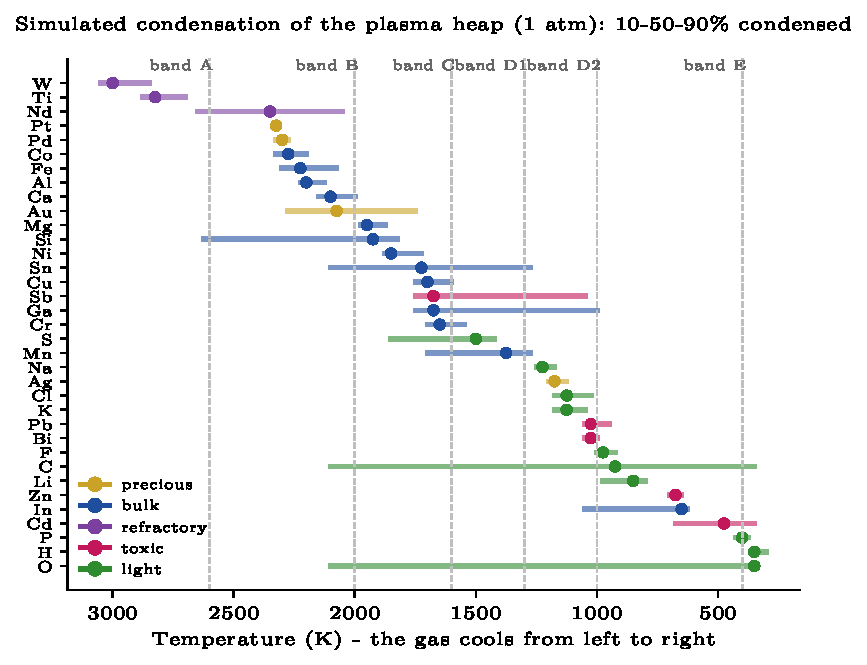
\includegraphics[width=0.86\textwidth]{figures/fig_ladder_simulated.pdf}
\caption{Simulated condensation at 1\,atm: temperatures at which 10\%, 50\% (dot) and 90\% of each element has condensed. Dashed lines mark the bands.}\label{fig:ladsim}
\end{figure}

\textbf{Gold, with full chemistry.} Chlorine stays as HCl in this hydrogen-rich gas, so the precious metals land in the same bands with the least and most volatile published chloride data. Palladium and platinum stay with iron. Gold divides between the iron band (58\%) and the copper band (42\%): iron condenses first, where gold's dislike of iron is weak (activity coefficient about 1.4--2.3 at 1,900--2,250\,K, extrapolated from \citealp{nagamori1968}), and the rest dissolves in the copper of Band C, which it prefers. Gold is enriched 28-fold in the metal of its main band (\gh{simulation/scripts/15_gold_copper.py}{15\_gold\_copper.py}), and both bands are alloys smelters already refine.

\textbf{What the evidence supports and corrects.} Table~\ref{tab:verdict} tests each claim of the original vision.

\begin{table}[!htbp]
\centering
\caption{Claims of the vision tested against the simulation (each backed by a script in the repository; see \gh{Results.txt}{Results.txt}).}\label{tab:verdict}
\footnotesize
\begin{tabular}{@{}p{4.2cm}p{7.6cm}p{1.9cm}@{}}
\toprule
\textbf{Claim} & \textbf{Simulation result} & \textbf{Verdict} \\
\midrule
All residue can be made gas & 2,890\,K at 1\,atm (2,630 at 0.1, 3,190 at 10\,atm) & Supported \\
Elements separate into bands & Clear bands, far below boiling points & Supported, revised \\
Precious metals concentrate & Pd, Pt with Fe; Au split B/C, 28-fold enriched & Supported, revised \\
Toxic volatiles leave the gold & No Zn, Hg, Pb in gold bands (5,000 feeds, pure phases, at equilibrium; fume carry-over not modelled); Cd $\le$0.01\%; Pb only after Band D split & Supported at equilibrium \\
The heap is its own reductant & Iron 100\% metal with the organics, 43\% without (\gh{simulation/scripts/03_reductant.py}{03\_reductant.py}) & Supported \\
Mercury gathers at the cold end & 58\% still gaseous at 300\,K (1\,atm); needs a trap & Revised \\
About 10.5\,MWh per tonne & 2.9\,MWh to all gas; 10.5 is an upper bound & Revised down \\
Bands sit at fixed temperatures & Every band moves with pressure; run at 1\,atm or above & Revised \\
The heap is a plasma & 0.02\% ionized at 2,890\,K: a torch-heated vapor & Revised \\
A sealed batch can cool slowly & Walls radiate the batch energy in seconds & Not supported \\
\bottomrule
\end{tabular}
\end{table}

Three findings change the design: band boundaries come from simulation and measurement, not boiling points; a mercury trap is a required outlet; and precious-metal enrichment is real but modest, so the Band B and C metal still goes to refining.

\textbf{How waste comes apart, and how fast.} Polymers crack long before the hot zone. PVC releases HCl at 272--379\,\textdegree C, and polyolefins decompose at 430--505\,\textdegree C \citep{yuan2020}. Molecules break in microseconds (CF\textsubscript{4} above). The slow step is heating mineral grains, which by heat conduction needs at least
\begin{equation}\label{eq:vaptime}
t = \rho\, d_0^2\,\big(\Delta h/12 + L/8\big)\big/\big(S_{\mathrm{gas}} - S_{\mathrm{surface}}\big),
\end{equation}
where $S = \int k\,dT$ is the conduction potential \citep{chen1988} (\gh{simulation/scripts/13_breakdown.py}{13\_breakdown.py}). In gas at 3,500\,K, silica grains up to 27\,\textmu m vaporize in 10\,ms and up to 43\,\textmu m in 25\,ms; measurements are less generous \citep{gitzhofer1996}, so the mineral fraction is ground to about 20\,\textmu m (1\% of the plasma energy; Section~\ref{sec:practical}) or heated as a molten film. European law holds incinerator gas at 850\,\textdegree C for two seconds \citep{eu2010ied}; PARAMANU is far hotter for milliseconds, and grain heating, not chemistry, sets the time.

\textbf{Robustness.} Each of 5,000 feeds draws every component mass (lognormal, 30\%), the trace and mercury contents (60\%), pre-treatment (0--30\%), pressure (0.1, 1 or 5\,atm), every activity coefficient within its uncertainty and one of three chloride data sets, and runs the full ladder from 6,000 to 300\,K: 570,000 equilibrium states, every one certified (Section~\ref{sec:certificate}; \gh{simulation/scripts/06_sweep.py}{06\_sweep.py}, \gh{simulation/scripts/12_sweep_analysis.py}{12\_sweep\_analysis.py}, all feeds in \gh{simulation/results/sweep_5000.csv}{sweep\_5000.csv}). Zinc, mercury and lead reached a gold band in none of them, a failure rate below 0.06\% at 95\% confidence (rule of three), and cadmium stayed at or below 0.01\% (Table~\ref{tab:sweep}). Pressure sets gold's split, as Result~3 predicts, so the plant should run at 1\,atm or above. Palladium and platinum stay with iron in 95\% and 94\% of feeds, and the chloride data barely matter (gold's median Band B share 61, 58 and 61\%). Halving the temperature step moves gold's Band B share by one point (\gh{simulation/scripts/09_convergence.py}{09\_convergence.py}). With an ideal liquid alloy (\gh{simulation/scripts/11_alloy_model.py}{11\_alloy\_model.py}) nickel joins iron and Band B becomes an iron--nickel--copper alloy of the kind refineries process, holding 0.009\% of the zinc and 0.5\% of the lead. The sweep ran in 0.41\,h on one rented cloud server for under one US dollar, so anyone can repeat it.

\begin{table}[!htbp]
\centering
\caption{The 5,000-feed sweep by operating pressure.}\label{tab:sweep}
\footnotesize
\begin{tabular}{@{}p{6.2cm}rrrr@{}}
\toprule
& \textbf{0.1\,atm} & \textbf{1\,atm} & \textbf{5\,atm} & \textbf{All} \\
\midrule
Gold mainly in Band B / C / D1 (\% of feeds) & 1 / 59 / 40 & 74 / 26 / 0 & 99 / 0 / 0 & 58 / 28 / 14 \\
Gold in Bands B and C, 5th percentile (\%) & 40 & 99 & 72 & 46 \\
Zinc, mercury or lead in a gold band & none & none & none & none \\
Median mercury still gaseous at 300\,K (\%) & 100 & 58 & 10 & 62 \\
\bottomrule
\end{tabular}
\end{table}

\textbf{Benchmarks and limits.} Lead and tin vapor pressures match the vacuum-refining literature within 3\% and 9--18\% \citep{jia2013} (\gh{simulation/scripts/14_benchmarks.py}{14\_benchmarks.py}). The model reproduces measured iron metallization of carbon-reduced steel-mill dust \citep{chang2022}, where biomass releasing its reductant as gas removed 97.9\% of the zinc, near the equilibrium ceiling, as the heap's gas-phase reductant should. Measured gold partition between liquid iron and copper \citep{yamaguchi2006} shows the model overstates gold's preference for copper by 2--4 times, erring against the iron band. The model assumes equilibrium, pure oxides and ideal alloys, and no nucleation or aerosol carry-over, and the gold--iron coefficient is extrapolated; these limits are bracketed in the sweep and named as experiments (Section~\ref{sec:feasibility}). Next computational steps: CALPHAD solution models, reacting-flow simulation and machine-learned data for missing species, on GPU servers.

\section{Rechecking the Computation}\label{sec:verification}

The sweep shows the claims survive variation \emph{if the model is right}; this section tests the model itself, each time with a check that does not share the weakness it checks. The checks found three defects in the computation and one in the design; all are reported and fixed, and every number was recomputed.

\subsection{A Certificate for Every Equilibrium State}\label{sec:certificate}
Result~2 also says how to \emph{recognize} the equilibrium without trusting the solver that found it \citep{boyd2004}. A state with gas amounts $n_k$ and condensed amounts $n_c$ is the equilibrium if and only if one vector $\lambda$ satisfies
\begin{align}
\ln x_k &= a_k\cdot\lambda - g_k - \ln(P/P_0) && \text{every gas species}, \label{eq:cert1}\\
a_c\cdot\lambda &= g_c \ \text{(phase present)}, \qquad a_c\cdot\lambda \le g_c \ \text{(phase absent)}, && \label{eq:cert2}\\
\textstyle\sum_k a_{ik} n_k + \sum_c a_{ic} n_c &= b_i && \text{every element}. \label{eq:cert4}
\end{align}
The certificate fits $\lambda$ by least squares from the amounts alone and demands every condition to $10^{-4}$. Since the equilibrium is unique, a state that passes is \emph{the} equilibrium, whatever produced it. All 570,000 sweep states pass; the code is \texttt{certify} in \gh{simulation/paramanu_sim/equilibrium.py}{equilibrium.py}, and \gh{simulation/tests/test_ladder.py}{test\_ladder.py} checks every ladder step.

\subsection{What the Checks Found}\label{sec:defects}
\textbf{Unconverged steps.} Against Cantera, PARAMANU's solver had not converged at 43 of 229 ladder steps below 1,850\,K, because parts-per-billion remnants were solved with the majors; elements below one part per million of the gas now go to the dilute-limit solver, and nothing is dropped. \textbf{A solver that is confidently wrong.} At 0.1\,atm Cantera reported convergence (balance $10^{-15}$) for non-equilibrium states and, as a backup, put zinc and lead in the wrong bands in 183 feeds; the certificate rejects them by up to 168 in $\ln x$. A solver's report of convergence is not proof; the certificate decides. \textbf{A missing phase.} Graphite was supersaturated in rare carbon-rich states; the NASA CEA phase-set iteration now adds it, and the claims did not change. All three are logged with dates in \gh{Results.txt}{Results.txt}.

\subsection{Second Solver, Second Database, Second Machine}
A second, separately written solver (Cantera's VCS, \citealp{smithmissen1982}) found the same condensed phases at all 51 states where it converged, with amounts within 0.19\%. The full NASA CEA database (558 gas and 366 condensed species, independent NASA-9 fits) puts 21 of 23 elements in the same band (median change 0\,K), with iron, copper, nickel, zinc, lead and mercury identical. Twenty sweep feeds recomputed on a second computer match to $1.1\times10^{-13}$ with identical bands (\gh{simulation/scripts/18_independent_verification.py}{18\_independent\_verification.py}, \gh{simulation/scripts/19_reproducibility.py}{19\_reproducibility.py}).

\subsection{An Adversary}\label{sec:falsification}
A rare failure can hide between random samples, so differential evolution \citep{storn1997} (\gh{simulation/scripts/20_falsification.py}{20\_falsification.py}) searched all 56 uncertain inputs, over wider ranges than the sweep, for a feed that moves a toxic volatile metal into a gold band. \textbf{Against the first design it broke the lead claim}: in 162 of 1,664 attempts over 1\% of the lead reached a gold band. It took two to three times the usual paper and plastics, whose gases dilute the metal vapor, so gold condensed later and partly passed into Band D (then 1,000--1,600\,K), where lead collects. The band was too wide; lead never moved toward the gold. The stray gold condenses above 1,300\,K and the lead below, with a 550\,K gap, so Band D was split at 1,300\,K into D1 and D2 and the search rerun: in 6,656 feeds no zinc, mercury or lead reached a gold band, and cadmium stayed at or below 0.025\%.

\subsection{Which Uncertainties Matter}\label{sec:sobol}
First-order Sobol indices \citep{sobol2001,plischke2013} (\gh{simulation/scripts/21_global_sensitivity.py}{21\_global\_sensitivity.py}) show that pressure, an operating choice, explains 58--84\% of the variance of every gold and mercury result. At 1\,atm one uncertain input dominates: the activity coefficient of gold in liquid iron explains 86\% of the variance of gold's Band B share. \textbf{One measurement of that coefficient near 2,000\,K would remove most of the remaining uncertainty} (prediction P11).

\subsection{Predictions Registered Before Experiment}\label{sec:prereg}
The strongest test is one whose passing mark is fixed before the measurement \citep{nosek2018}. Table~\ref{tab:prereg} registers the predictions for the first experiments, also fixed in \gh{docs/PREREGISTRATION.md}{docs/PREREGISTRATION.md} (to be deposited with a timestamped DOI at submission). P1 and P2 are consistency checks; P3--P13 are risky tests.

\begin{table}[!htbp]
\centering
\caption{Predictions registered before experiment (default synthetic residue, 1\,atm unless stated).}\label{tab:prereg}
\footnotesize
\begin{tabular}{@{}l>{\raggedright\arraybackslash}p{5.6cm}>{\raggedright\arraybackslash}p{3.0cm}>{\raggedright\arraybackslash}p{4.0cm}@{}}
\toprule
& \textbf{Prediction} & \textbf{Passes if} & \textbf{Counts against if} \\
\midrule
P1 & Every element balance closes (Result~1) & within 3 std.\ unc. & it does not \\
P2 & Energy to all gas $\geq$ 2.90\,MWh per wet tonne & $\geq$ 2.6\,MWh/t & below 2.6\,MWh/t \\
P3 & Iron in Band B is metal & $\geq$90\% metallic & $<$50\% metallic \\
P4 & T50 order Fe 2,225 $>$ Au 2,075 $>$ Cu 1,700 $>$ Pb 1,025 $>$ Zn 675 $>$ Cd 475\,K & order kept; Fe, Cu, Pb, Zn within 150\,K & Zn, Cd or Hg above Au or Cu; or off by $>$150\,K \\
P5 & No Zn, Hg or Pb in bands holding $\geq$10\% of the gold & $<$1\% of each & $\geq$1\% of any \\
P6 & Cadmium in those bands $\leq$0.01\% & $<$0.1\% & $\geq$0.1\% \\
P7 & Gold in Bands B+C: 100\% & $\geq$95\% & $<$90\% \\
P8 & Gold in Band B: 58\% (feeds: 40--83\%) & 20--95\% & outside 20--95\% \\
P9 & Pd and Pt in Band B: $\sim$100\% & $\geq$90\% & $<$70\% \\
P10 & 1 to 5\,atm raises gold's T50 ($\sim$250\,K) and B share & both rise & either falls \\
P11 & $\gamma$ of gold in liquid iron, 1,900--2,250\,K: 1.4--2.3 & 0.5--7 & outside: P8 recomputed \\
P12 & CF\textsubscript{4} destroyed at $\geq$2,600\,K in 25\,ms & $<$0.01\% leaves & $\geq$0.01\% leaves \\
P13 & Organic-rich adversary feed: gold in D1, lead in D2 & $<$1\% overlap each & $\geq$1\% of either \\
\bottomrule
\end{tabular}
\end{table}

\begin{table}[!htbp]
\centering
\caption{The rechecks at a glance.}\label{tab:verification}
\footnotesize
\begin{tabular}{@{}>{\raggedright\arraybackslash}p{3.4cm}>{\raggedright\arraybackslash}p{4.0cm}>{\raggedright\arraybackslash}p{6.4cm}@{}}
\toprule
\textbf{Test} & \textbf{Would catch} & \textbf{Result} \\
\midrule
Certificate (Result~2) & any non-equilibrium state & all 570,000 sweep states pass \\
Second solver & solver errors & same phases at all 51 shared states \\
Second database & data errors & 21 of 23 elements in the same band \\
Published measurements & wrong data or chemistry & vapor pressures, metallization, gold partition \\
Adversarial search & rare failures & broke the first design for lead; none after the split \\
Sobol indices & hidden dependences & one coefficient decides gold's split; pre-registered \\
Second machine & hardware or software effects & agreement to $1.1\times10^{-13}$ \\
Pre-registration & fitting after the fact & 13 predictions fixed in advance \\
\bottomrule
\end{tabular}
\end{table}

\section{Energy, and Paying for It}\label{sec:energy}

\textbf{How much.} Turning one wet tonne of residue into gas at 2,890\,K takes a gross \textbf{2.9\,MWh} before heat recovery (\gh{simulation/scripts/04_energy.py}{04\_energy.py}); full atomization at 5,000\,K would take 10.5\,MWh, an upper bound (drying 0.2, soil and glass 4.0, plastics 3.2, paper and wood 1.3, heating the atoms 1.75\,MWh; ionizing a tenth would add 2.1). A 1,000-tonne-per-day plant draws about 120\,MW (113\,MW with drying by waste heat). The best demonstrated plasma vaporization of silica, a centrifugal furnace with carbon, needed 9.3\,kWh/kg, about 2.3 times the gross enthalpy \citep{sayce1976}, or about 280\,MW for the plant; so heat a molten film or bath directly rather than blowing powder through a torch jet, and grind injected powder fine (Eq.~\ref{eq:vaptime}). Pre-treatment is a moderate dial: removing 30\% of the mass lowers the energy from 3.0 to 2.5\,MWh per tonne. Most energy returns, as condenser heat and as fuel gas; recovered as steam in boiler walls, the heat yields 0.41--0.55\,MWh of electricity per tonne, 14--19\% of the gross (Section~\ref{sec:practical}). The torches need firm power from a \textbf{dedicated power plant} (gas with carbon capture, renewables with storage, or nuclear, as a power source only), and the environmental case stands or falls with it.

\textbf{Its own fuel.} The hydrogen, carbon monoxide and methane drawn off can drive a fuel cell or turbine, and iron, aluminium, silicon and magnesium powders are studied as recyclable metal fuels that burn to oxides without carbon dioxide. Such fuels return only part of the energy, since every unit they release was spent to recover them.

\textbf{Paying for the rest: selling what it recovers.} The harvested elements, sold pure or as usable compounds (metals, silica, alumina, salts, lithium carbonate), pay for part of the power (\gh{simulation/scripts/23_self_sufficiency.py}{23\_self\_sufficiency.py}). Valued at the Sort-First spreadsheet's prices, with unpriced elements at zero and bulk minerals at \$5 per tonne, one tonne yields about \textbf{\$113}, led by gold (\$39), copper (\$21), iron (\$12), chromium (\$8) and silver (\$8). \textbf{At today's best demonstrated heating efficiency, fuel and sales cover 36--43\% of the power bill at 5 cents per kWh, and 42--51\% with the condenser heat recovered as steam} (\gh{simulation/scripts/24_heat_recovery_and_scale.py}{24\_heat\_recovery\_and\_scale.py}). The plant becomes \textbf{self-sustaining} only near the gross enthalpy, about twice as efficient as demonstrated: there the sales pay for the power it must buy at up to 4--5 cents per kWh, and with steam recovery it covers 97--118\% of its energy at 5 cents. Self-sufficiency is a target, not a result; efficient heating (R5) is the economic key. The account omits capital, refining, argon, grinding and labour, and also gate fees and avoided remediation; and gold, its largest item, has an assumed content.

\section{What One City Landfill Holds}\label{sec:landfill}

The median US municipal landfill holds 2.3 million tonnes of waste (our calculation from 2,175 landfills in the EPA database; \citealp{epa2024lmop}), six years for a 1,000-tonne-per-day plant. With simulated band capture and established refining yields \citep{hageluken2010,cusano2017bref} (\gh{simulation/scripts/16_landfill_inventory.py}{16\_landfill\_inventory.py}), it could return about 196 million lb of iron, 12.0 million lb of copper, 6.0 million lb of zinc, 1.7 million lb of nickel, 32,000 lb of silver, 1,800 lb of gold, 720 lb of palladium and 180 lb of platinum; 687 million lb of silicon as silica and glass and 170 million lb of aluminium as alumina; salts, lime, magnesia, phosphate and lithium carbonate; and it would capture 14,000 lb of cadmium and all 7,600 lb of mercury. (Precious-metal contents are assumed: 0.5, 0.2 and 0.05\,ppm.)

\textbf{What remains is made safe for centuries.} Off-specification condensate returns to the feed, losing nothing (Results~1 and~7). The mineral remainder becomes glass, the most durable common waste form: a reference waste glass would take over 250,000 years to corrode one centimetre \citep{gin2015}. Toxic elements are stored in forms nature has kept for geological time: mercury as mercury sulfide (cinnabar), as European law requires \citep{eu2017mercury}, cadmium as sulfide and fluorine as fluorite (Table~\ref{tab:storage}).

\begin{table}[!htbp]
\centering
\caption{Storage form of recovered elements: pure where stable and sold that way, otherwise a stable compound.}\label{tab:storage}
\footnotesize
\begin{tabular}{@{}p{3.3cm}p{5.2cm}p{5.4cm}@{}}
\toprule
\textbf{Form} & \textbf{Elements} & \textbf{Stored as} \\
\midrule
Pure metal & Fe, Al, Cu, Zn, Pb, Ni, Co, Sn, Bi, In, Ga & ingots, cathodes, alloy \\
Precious metal & Au, Ag, Pd, Pt & bullion, sponge \\
Reactive element & Li, Na, K, Ca & Li\textsubscript{2}CO\textsubscript{3}, NaCl, KCl, CaSO\textsubscript{4} \\
Hazardous gas & F, Cl, N, P & CaF\textsubscript{2}, NaCl, ammonium sulfate, phosphate \\
Toxic element & Hg, Cd, As, Cr & HgS, CdS, scorodite, Cr\textsubscript{2}O\textsubscript{3} \\
\bottomrule
\end{tabular}
\end{table}


\section{Operating Policy, Comparison and Safety}\label{sec:safety}

\textbf{What is worth purifying.} Atomizing everything does not mean purifying everything.

\begin{definition}[Value--harm criterion]
With market value $V_i$, monetized harm $H_i\ge 0$ if left in the environment, recovery cost $C_i$ from the band condensate, and an operator's slider $s\in[0,1]$, element $i$ is purified if and only if $V_i + s\,H_i > C_i$, and is otherwise vitrified as future ore.
\end{definition}
\begin{proposition}[Monotone activation]\label{prop:mono}
For $H_i>0$, element $i$ is purified exactly for $s > s^\ast_i = (C_i - V_i)/H_i$, so the set of purified elements, and the harm avoided, never shrink as $s$ moves from 0 (Commercial) to 1 (Nature).
\end{proposition}
\begin{proof}
$V_i + sH_i$ is non-decreasing in $s$, so an element purified at $s$ is purified at every $s'>s$.
\end{proof}
Since cost follows the Sherwood relation \citep{sherwood1959,johnson2007} and the band condensate is far richer than the heap, the ladder lowers $C_i$ for every element it concentrates. With the baseline's illustrative inputs (Figure~\ref{fig:slider}; \gh{model/paramanu_mass_energy_balance.xlsx}{baseline spreadsheet}), mercury, cadmium and chromium switch on almost at once, arsenic at $s^\ast\approx0.105$ and fluorine at $s^\ast\approx0.716$. The operator can therefore choose, band by band, between profit and protection of nature.

\begin{figure}[!htbp]
\centering
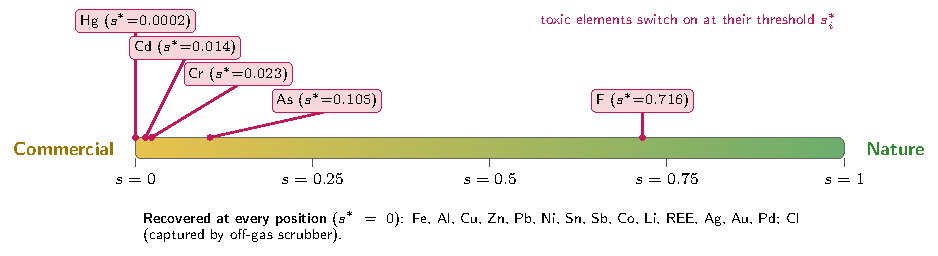
\includegraphics[width=0.74\textwidth]{figures/fig_slider.pdf}
\caption{Activation thresholds $s^\ast_i$ on the Commercial--Nature slider (illustrative inputs from the Sort-First baseline model).}\label{fig:slider}
\end{figure}

\textbf{Against a Sort-First baseline.} A \gh{model/paramanu_mass_energy_balance.xlsx}{spreadsheet model} of a conventional plant (pre-sorting, plasma gasification, refining, vitrification) needs 0.26--0.54\,MWh per tonne, recovers 15--20 elements, and earns \$30--52 per tonne while avoiding \$113--231 of monetized harm, depending on the slider; it recovers only what sorting reaches. Atomize-First needs 5--11 times its electricity, but removes the dependence on sorting, treats the residue every other process leaves, and has no process stack (Table~\ref{tab:compare}).

\begin{table}[!htbp]
\centering
\caption{Sort-First against Atomize-First.}\label{tab:compare}
\footnotesize
\begin{tabular}{@{}p{3.1cm}p{5.2cm}p{5.6cm}@{}}
\toprule
 & \textbf{Sort-First (baseline)} & \textbf{Atomize-First (PARAMANU)} \\
\midrule
Input & Sorted streams & Residue after optional pre-treatment \\
Separates & Objects and materials & Atoms \\
Separation physics & Magnetism, density, optics, chemistry & Condensation temperature, mass, chemistry \\
Off-gas & Cleaned and released through a stack & No process stack: sealed flow reactor, labelled outlets (fuel use and power plant have their own) \\
Toxic elements & Captured where chemistry allows & Zn, Cd, Pb condense far from the gold; Hg to a trap \\
Trace elements & Lost when too dilute & Concentrated with the band metal (Au 28-fold) \\
Energy (MWh/t) & 0.26--0.54 & 2.9 (all gas) to 10.5 (full atomization), gross \\
Maturity & Commercial components & Research concept \\
\bottomrule
\end{tabular}
\end{table}

\textbf{Carbon and safety.} No process stack is not zero impact: it moves to the power plant and wherever the fuel is burned, and a life-cycle assessment \citep{iso14040,iso14044} must decide. Electricity dominates: at 2.9--6.7\,MWh per tonne, unabated gas combined-cycle power (life-cycle median about 490\,g CO\textsubscript{2}/kWh; \citealp{schlomer2014}) means about 1.4--3.3\,t CO\textsubscript{2} per tonne of waste, likely more than landfilling or incineration, and nuclear or wind power (about 12\,g/kWh) about 0.03--0.08\,t. \textbf{PARAMANU is an environmental gain only on low-carbon power.} Pressure is relieved only into closed volumes, and a hazard study must cover fuel gas and air ingress, metal carbonyls at the cold end, pyrophoric fume, acid condensate and torch power. \textbf{Nuclear and radiological materials} (uranium, thorium, plutonium, radium, polonium, sealed-source isotopes) are excluded from every inventory and design here: their recovery belongs only in licensed, regulated facilities, and landfills hold them only at trace, soil-like levels. Radioactive items are diverted before the plasma. Because the process fractionates every element, the soil's natural radionuclides will be redistributed (uranium and thorium oxides to Band~A, lead-210 and polonium-210 to the cold bands), so a band-by-band mass balance is required before operation \citep{nrc10cfr40}.

\section{What Is Proven, What Is Verified, What Is Open}\label{sec:feasibility}

The paper offers three kinds of evidence, each to be held to its own standard.

\textbf{Tier 1: proven.} Results~1--4 and 6--8 are established results of thermodynamics and convex optimization under stated assumptions (ideal gas, equilibrium at each step, pure phases or ideal solutions); Result~5 is an order-of-magnitude estimate on a rigorous geometric bound. A critic may dispute the assumptions, not the conclusions that follow from them.

\textbf{Tier 2: verified.} The simulation computes what thermodynamics predicts for this waste from the most trusted data \citep{mcbride2002,chase1998}, and a certificate, a second solver and database, published measurements, an adversary and a second machine show it does so correctly; its defects are published with their fixes.

\textbf{Tier 3: not yet proven.} Whether a real reactor behaves like the model. Five effects can break it: fume and aerosols carried past their condenser (the largest threat to band purity), kinetics and nucleation, non-ideal alloys and slag, a uniform 25\,ms hot zone at scale, and energy efficiency. Only experiments can close this gap.

The claim is therefore \textbf{thermodynamic feasibility with a verified computation}, not a working plant. Four practices make it checkable: failures and corrections are published with dates (\gh{Results.txt}{Results.txt}); every number regenerates from public code with pinned library versions; predictions are fixed before measurement; and untested assumptions are named. The deciding experiment suits a university laboratory: a sealed arc furnace, a few kilograms of synthetic residue and condensers at the band temperatures. Three predictions carry the weight: iron collected as metal (P3), the predicted order of condensation (P4), and no zinc, mercury or lead with the gold (P5). If they pass, the question becomes how to scale; if they fail, the fixed marks show which assumption broke.

\begin{table}[!htbp]
\centering
\caption{Research agenda, in the order we would attack it.}\label{tab:agenda}
\footnotesize
\begin{tabular}{@{}lp{4.3cm}p{8.9cm}@{}}
\toprule
\textbf{No.} & \textbf{Question} & \textbf{First experiment} \\
\midrule
R1 & Do elements condense as metals? & Sealed bench arc furnace, synthetic residue; analyse each collector at several cooling rates \\
R2 & How clean is each band? & Cross-contamination between bands; fume and aerosol carry-over \\
R3 & Can a mass filter split co-condensing groups? & Couple a small plasma mass filter to a Band B/C vapor stream \\
R4 & Can the hot zone be built? & Sealed flow reactor: residence time, wall flux ($\sim$1\,MW\,m\textsuperscript{-2}), skull stability, gas curtain, the three flow conditions \\
R5 & How much energy, and how much returns? & Transferred-arc and centrifugal furnaces vs powder injection; boiler-wall steam recovery from the condenser stages \\
R6 & Does pre-treatment change quality? & Repeat R1 at 0, 15 and 30\% pre-treatment \\
R7 & Can the heap be monitored live? & Optical emission spectroscopy during vaporization and cooling \\
R8 & Does it scale? & Flow or pulsed reactor from 1\,kg/h to 1\,t/h \\
R9 & How good is the model? & Measure $\gamma$ of gold in liquid iron (P11); CALPHAD alloys and slag; nucleation and reacting-flow simulation \\
\bottomrule
\end{tabular}
\end{table}

\section{Conclusion}

This paper introduced \textbf{Atomize-First recovery} and the \textbf{PARAMANU Reclaimer}, resting on four ideas: the \textbf{closed-mass principle}, the \textbf{condensation ladder} laid out along a sealed flow train, the \textbf{internal reductant} supplied by the waste, and a \textbf{value--harm policy} for what to purify. PARAMANU changes three things. \textbf{It reverses the order}: it atomizes first, so the residue that ends every other process is where it begins. \textbf{It closes the loop}: a sealed reactor with no process stack, every atom through a labelled outlet, toxic volatile metals far from the gold and mercury in a trap. \textbf{It tests itself}: eight results with proofs, an open simulation that confirms and corrects the vision, and rechecks that found and fixed its defects. The mathematics is proof, the computation is verified evidence, and the working plant awaits an experiment whose passing marks are already fixed.

\begin{keyinsight}
\textbf{The residue where sorting ends is not the end of recycling, but the start of atomic recovery.} Once waste is taken apart into atoms in a sealed vessel, the question is no longer which object is which, but which element is which, and physics can tell elements apart.
\end{keyinsight}

For the thinkers who first imagined matter as \emph{param\={a}\d{n}u}, the atom was the smallest building block of the world. PARAMANU applies that idea to the waste we have buried: take it apart completely, keep what is valuable, lock away what is harmful, and vent nothing to the air. What was mined once is harvested again.

\section*{Data and Resources}
\addcontentsline{toc}{section}{Data and Resources}
All is public at \url{https://github.com/syncaissa/paramanu-reclaimer}: solver, ladder, 24 experiment scripts regenerating every number and figure, all 5,000 sweep feeds, 38 tests, the Sort-First spreadsheet, and cloud scripts. \gh{Results.txt}{Results.txt} lists every result and correction, \gh{HOWTOREPLICATE.txt}{HOWTOREPLICATE.txt} explains how to reproduce them, \gh{docs/IMPLEMENTERS_GUIDE.md}{docs/IMPLEMENTERS\_GUIDE.md} expands Appendix~A, and \texttt{AllExplainedHere.pdf} gives every derivation, table and worked example behind this paper.

\section*{Appendix A: Implementer's Guide}\label{sec:guide}
\addcontentsline{toc}{section}{Appendix A: Implementer's Guide}
{\small Ten steps turn the results into a design; examples are for 1,000 wet tonnes per day at 1\,atm with the default feed (replace with site data).
\begin{enumerate}[label=\textbf{A.\arabic*},leftmargin=2.6em,itemsep=2pt]
\item \textbf{Characterize the feed.} Sample across depth and area; measure moisture, organics (loss on ignition), majors (XRF) and traces (ICP-MS); enter them in \gh{simulation/paramanu_sim/feed.py}{feed.py}. \emph{Example:} 250\,kg water and 711\,kg dry residue per wet tonne.
\item \textbf{Make hazards safe} (mandatory): discharge batteries, depressurize cylinders and cans, divert radioactive items to a licensed handler.
\item \textbf{Compute the all-gas state} (\gh{simulation/scripts/04_energy.py}{04\_energy.py}): temperature $T$, specific energy $e$ and gas yield $\nu$. \emph{Example:} 2,890\,K, 9.8\,MJ/kg, 35.1\,mol/kg.
\item \textbf{Choose the pressure.} Higher pressure shrinks the hot volume and condenses more mercury; below 1\,atm gold moves to cooler bands (Result~3). \emph{Example:} 1\,atm in the hot zone, 2\,atm or more at the mercury trap.
\item \textbf{Size the hot zone} from Eq.~\ref{eq:flowloss}: pick the allowed radiation loss, solve for $t_r$, then $V = \dot m\,\nu RT t_r/P$. \emph{Example:} 96\,m\textsuperscript{3}/s of gas; 10\% loss gives $t_r = 25$\,ms, $V = 2.4$\,m\textsuperscript{3}, 126\,MW of torch power.
\item \textbf{Design the condenser train} (\gh{simulation/scripts/02_ladder.py}{02\_ladder.py}): one stage per band, set by Eq.~\ref{eq:onset} at the chosen pressure; size each exchanger from its duty, and use Eq.~\ref{eq:fenske} where a band must be split further. Build each stage as a boiler wall that raises steam, and follow it with a fume filter that returns its catch to that stage (Sections~\ref{sec:fume} and~\ref{sec:practical}). \emph{Example:} 13.6, 28.3, 21.9, 3.3, 11.5 and 15.7\,MW for stages A, B, C, D1, D2 and E.
\item \textbf{Capture mercury} with a sulfur-impregnated carbon bed after the coldest stage \citep{korpiel1997}, sized for all of the mercury input; store it as HgS.
\item \textbf{Route each band to refining.} Each collector is a settling hearth (metal under slag, tapped separately). B and C (iron and copper alloys with the gold, palladium and platinum) go to precious-metal smelting and electrorefining \citep{cui2008}. D1 goes with C. From D2, leach the salts and recover silver and lead; from E, split zinc and cadmium. Keep D1 and D2 in separate collectors. Convert toxic products to the forms of Table~\ref{tab:storage}; vitrify what the slider does not purify.
\item \textbf{Pass the acceptance tests}: element balances close (Eq.~\ref{eq:closedmass}); onsets match Result~3; band compositions match the model or the gap is explained; mercury is below the permit limit; energy and wall losses match Results~5 and~6; predictions (Table~\ref{tab:prereg}) are reported.
\item \textbf{Operate safely.} Relieve pressure only into closed volumes; interlock torches on pressure and wall temperature; keep radiation monitors at the intake (Section~\ref{sec:safety}).
\end{enumerate}}

\renewenvironment{pclosing}{\par\vspace{4pt}\centering\rule{0.5\textwidth}{0.4pt}\par\vspace{2pt}\small}{\par}
\begin{pclosing}
Syncaissa Systems Inc. \quad $\bullet$ \quad \texttt{syncaissa@outlook.com}\\[2pt]
\url{https://github.com/syncaissa/paramanu-reclaimer}
\end{pclosing}

{\footnotesize\linespread{0.94}\selectfont
\bibliographystyle{apalike}
\setlength{\bibsep}{0pt}
\setlength{\columnsep}{14pt}
\begin{multicols}{2}
\bibliography{references}
\end{multicols}
}



\end{document}
